

\fancypagestyle{miEstilo503}{
   \lhead{5.3 Interacción entre componentes y servicios}
   \rhead{Página \thepage}
   \lfoot{}
   \cfoot{}
   \rfoot{}
}

\pagestyle{miEstilo503}


\subsection{Interacción entre componentes y servicios} \label{sec:interac}

En la sección anterior se ha descrito qué hace cada componente y qué funcionalidades aporta a la aplicación, pero ¿cómo interaccionan entre sí para llevar a cabo las distintas tareas? A continuación se van a describir algunas de las interacciones que se realizan entre los servicios para llevar a cabo una cierta tarea.

\textbf{Interacción entre el usuario y el bot de Telegram}

La interacción entre el usuario y el bot de Telegram es la siguiente:

\begin{figure}[H]
	\centering
	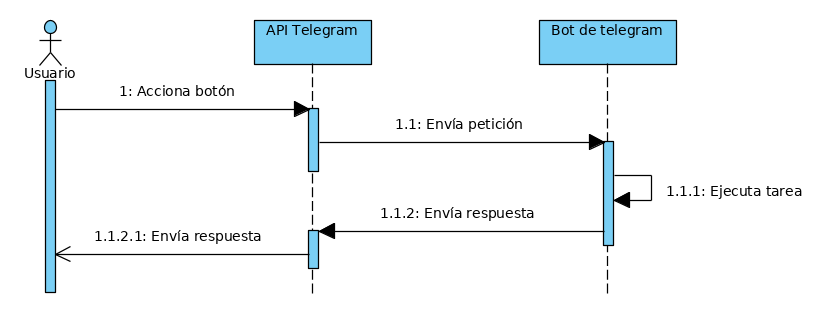
\includegraphics[scale=0.6]{images/84}
	\caption{Interacción usuario con el bot de Telegram}
	\label{f:1}
\end{figure}

Cuando el usuario acciona un botón en la interfaz del bot o envía un comando, dicho mensaje es enviado a la API de Telegram a la cual se conecta el Bot de Telegram gracias al \texttt{API Token}. Dicha solicitud es recibida por el bot desarrollado, que ejecuta la tarea y envía la respuesta a la API de Telegram, y esta a su vez la reenvía a la conversación del bot con el usuario.

\textbf{Proceso de autenticación en el bot de Telegram}

Como se ha podido observar en la figura \ref{f:1}, el usuario ha podido establecer una comunicación con el bot de Telegram, pero para ello es necesario que ese usuario esté registrado como usuario permitido.

En la siguiente figura vamos a observar como se realiza dicho proceso.

\begin{figure}[H]
	\centering
	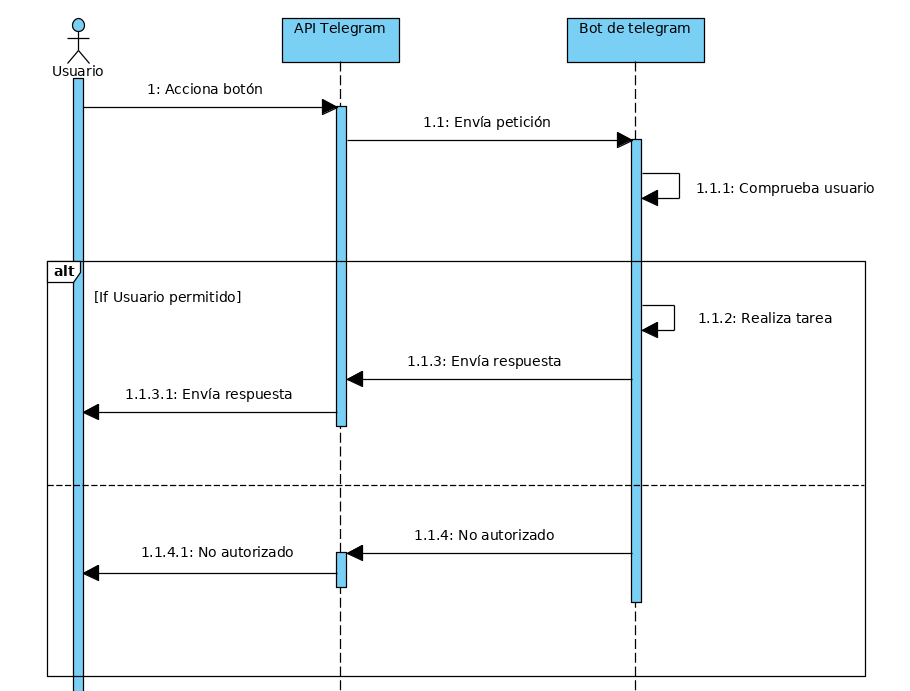
\includegraphics[scale=0.6]{images/85}
	\caption{Interacción usuario autenticado con el bot de Telegram}
	\label{f:2}
\end{figure}

Como se puede observar, cuando el usuario establece una comunicación con el bot, automáticamente se comprueba si dicho usuario está permitido, en cuyo caso se realiza la tarea y se le envía la respuesta. En caso contrario, se le enviará un mensaje diciéndole que no está autorizado.

\textbf{Proceso de autenticación en la API principal}

Una vez el usuario ha establecido comunicación con el bot de Telegram, es necesario que este bot junto con otros servicios se puedan comunicar con la \texttt{API} principal para poder realizar las tareas solicitadas.

Para poder establecer esta comunicación, la \texttt{API} dispone de un sistema de autenticación propio basado en un usuario y contraseña. Dicho usuario y contraseña será necesario adjuntarla junto con la petición a la \texttt{API} para poder establecer dicha comunicación satisfactoriamente.

\begin{figure}[H]
	\centering
	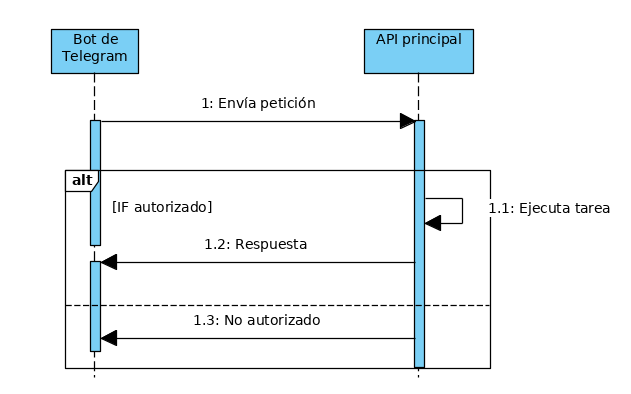
\includegraphics[scale=0.6]{images/86}
	\caption{Interacción entre el bot de Telegram y la API principal}
	\label{f:3}
\end{figure}

Al igual que en el caso anterior, solo se realizará la tarea si el servicio se ha autenticado correctamente, y en caso contrario, se devolverá un mensaje con código de estado 401 (No autorizado).

\textbf{Activación manual de la cámara o vídeo}

Cuando el usuario activa el modo manual para poder realizar una captura de una foto o la grabación de un vídeo, ocurre lo siguiente:

\begin{figure}[H]
	\centering
	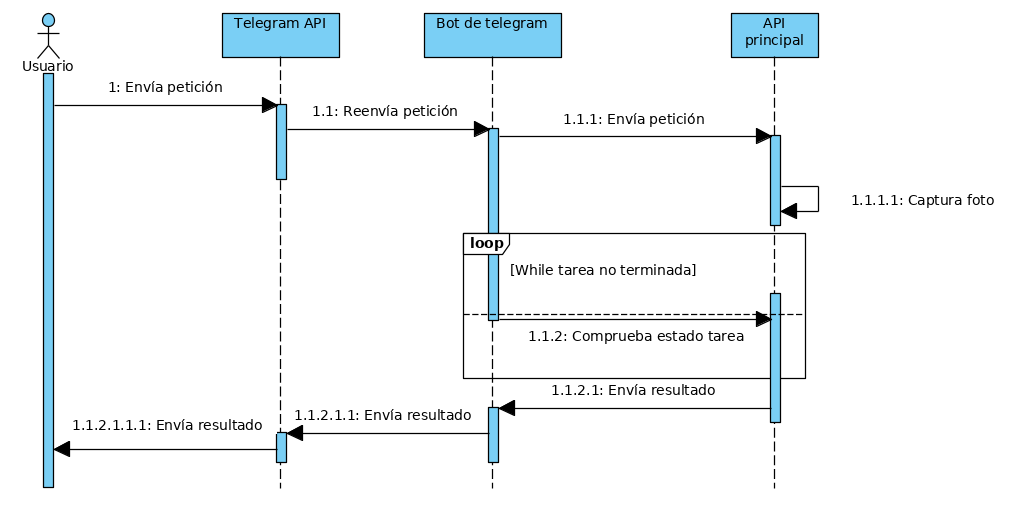
\includegraphics[scale=0.6]{images/87}
	\caption{Interacción entre servicios para realizar una foto}
	\label{f:4}
\end{figure}

Como se puede ver en la figura \ref{f:4}, el bot de Telegram envía la solicitud a la \texttt{API} principal y posteriormente envía periódicamente peticiones a la API para comprobar el estado de la tarea (ya que es asíncrona). Por otra parte, cuando la \texttt{API} recibe la petición para capturar la foto o grabar un vídeo, ésta crea una tarea asíncrona y la pone en cola para poder realizarla. Una vez que ha sido realizada, el bot de Telegram comprobará el estado finalizado y enviará el resultado (que es un mensaje más la imagen capturada) al usuario en la conversación que tiene con el bot.

\textbf{Activación del modo automático}

Cuando el usuario activa el modo automático para poder recibir alertas, ocurre lo siguiente:

\begin{figure}[H]
	\centering
	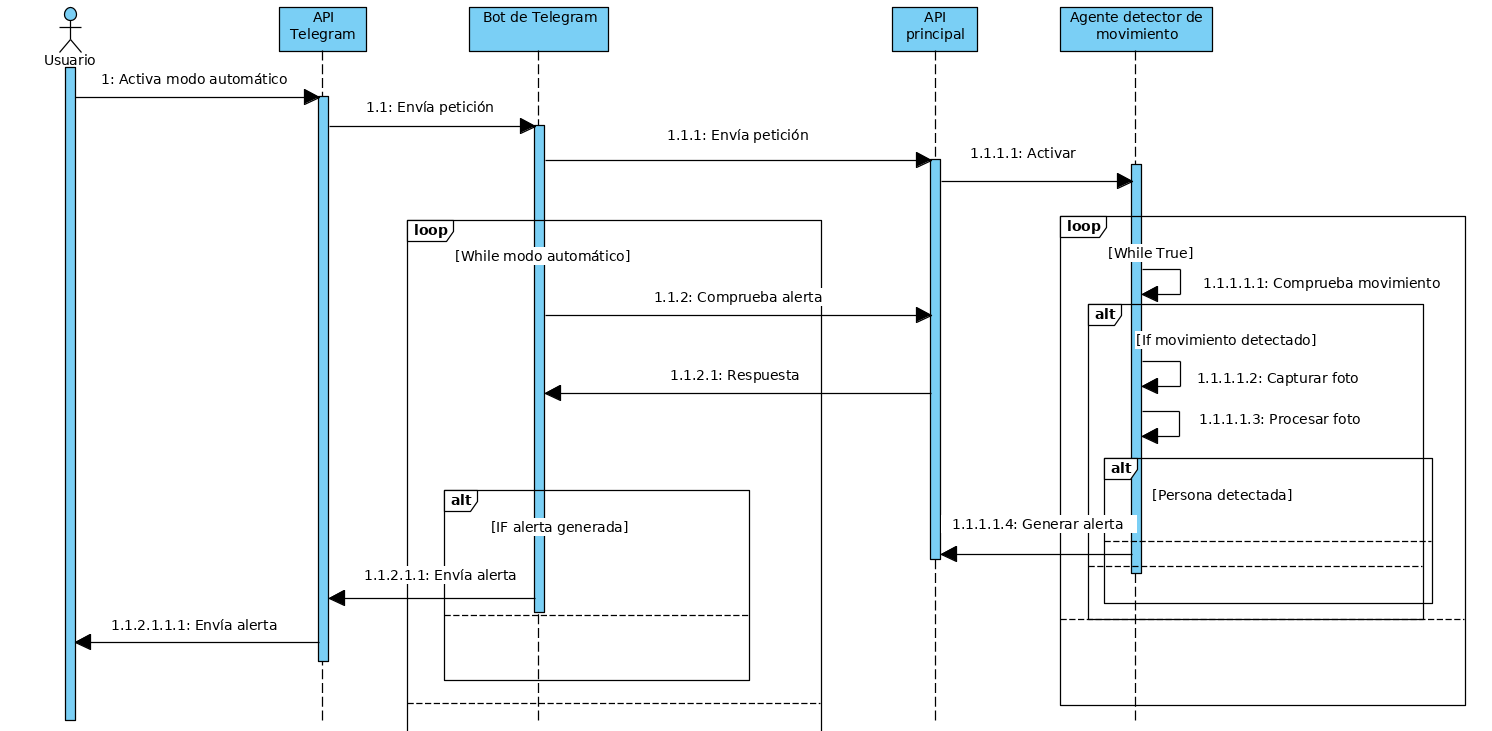
\includegraphics[scale=0.42]{images/88}
	\caption{Interacción entre procesos en el modo automático}
	\label{f:5}
\end{figure}

En primer lugar, la petición llega hasta la \texttt{API} que es la encargada de iniciar el proceso del agente detector de movimiento. A continuación, dicho agente estará en un bucle comprobando el estado del sensor. Cuando se ha detectado algún tipo de movimiento, entonces el agente detector de movimiento realizará una captura de imagen (o vídeo si prefiere) y a continuación pasa a procesar la foto (en el caso de estar habilitada dicha opción). Dicho procesamiento lo realizará el agente detector de objetos (que se detallará en el siguiente apartado) y devolverá la respuesta al agente detector de movimiento. En caso de que se haya detectado una persona, entonces se generará una alerta en la \texttt{API} principal para modificar su estado. Este estado es comprobado periódicamente por el Bot de Telegram, que en cuanto detecte la presencia de una alerta, enviará un mensaje junto con el archivo generado automáticamente (foto o vídeo) al usuario.

También, como observación adicional, se puede comprobar que el bot de Telegram permanece en un bucle realizando peticiones de comprobación a la \texttt{API principal}, pero esto no impide que el bot pueda procesar (en otra hebra) otro tipo de peticiones que se le envíen. De hecho, tiene que atender la petición de cambio de modo para que no se produzca ningún interbloqueo.

\textbf{Interacción entre el agente detector de movimiento y objetos}

Como se ha podido observar en el apartado anterior (ver figura \ref{f:5}), cuando se detecta una alerta de movimiento entonces realiza la captura de una foto y después se pasa a procesarla. El agente detector de objetos es el encargado de realizar este procesamiento. En la siguiente figura se puede observar este proceso.

\begin{figure}[H]
	\centering
	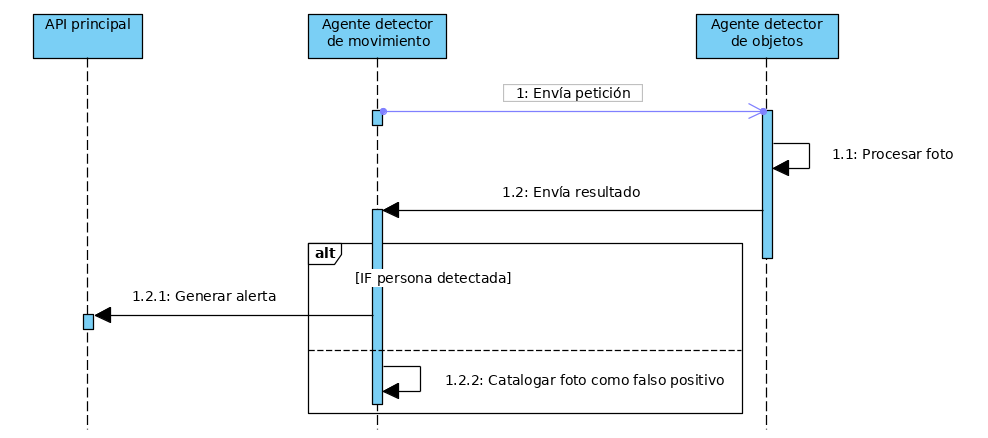
\includegraphics[scale=0.42]{images/90}
	\caption{Interacción entre el agente detector de movimiento y objetos}
	\label{f:6}
\end{figure}

En primer lugar, el agente detector de movimiento envía una petición asíncrona para procesar la foto capturada al agente detector de objetos. Es importante que esta petición sea \textbf{asíncrona}, ya que el procesamiento de la foto puede tardar entre unos 5 y 10 segundos y esto bloquearía al agente detector de objetos para poder seguir capturando posibles alertas.

En cuanto el agente detector de objetos recibe la respuesta, crea pone y en cola dicha tarea para poder ejecutarla. Tras finalizar su ejecución, enviará el resultado al agente detector de movimiento, que comprobará si en ese resultado se ha detectado a una persona. En el caso de detectar una persona, generará una alerta en la \texttt{API} principal, y en caso contrario, catalogará dicha alerta como falsa positiva (o no generará ninguna alerta en la \texttt{API}) y moverá la foto capturada al directorio de archivos falsos positivos.

\textbf{Activación manual del modo streaming}

Cuando el usuario activa el modo streaming para poder visualizar la retransmisión de vídeo en directo, ocurre lo siguiente:

\begin{figure}[H]
	\centering
	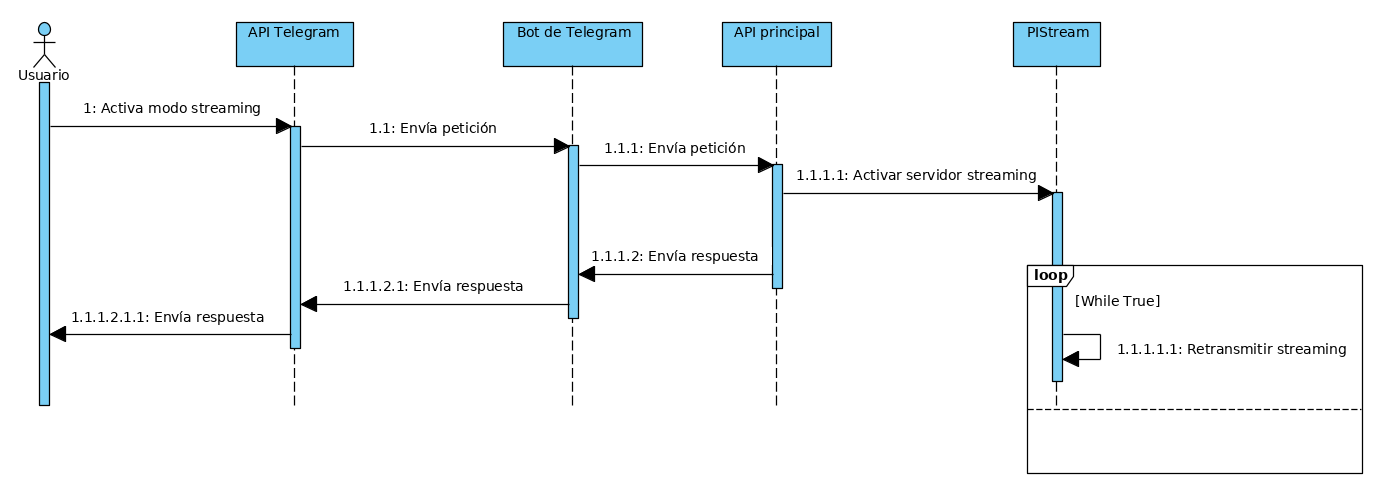
\includegraphics[scale=0.42]{images/89}
	\caption{Interacción entre procesos en el modo streaming}
	\label{f:7}
\end{figure}

En definitiva, el proceso es bastante similar que cuando se activa el modo manual para realizar una captura de una foto o la grabación de un vídeo. En este caso, la \texttt{API} principal se encarga de iniciar el servicio de streaming, que estará continuamente retransmitiendo los datos de vídeo hasta que se vuelva a cambiar de modo. Una vez que este servicio se ha activado, se le envía un mensaje al usuario para notificarle la URL donde podrá visualizar dicho streaming.